%Chapter 1 
\chapter{Measurement of the Left Right Asymmetry in the Drell-Yan Process} 
\label{Chap::setup}
\ifpdf
\graphicspath{{Chapters/OneCh/Figs/Raster/}{Chapters/OneCh/Figs/PDF/}{Chapters/OneCh/Figs/}}
\else \graphicspath{{Chapters/OneCh/Figs/Vector/}{Chapters/OneCh/Figs/}} \fi

Introduction about L/R asym.  In this Chapter....  Define AN

\section{Data Sample}
The data sample comes from the 2015 COMPASS Drell-Yan measurement where a 190
GeV/c $\pi^-$ beam impinged on a transversely polarized NH$_3$ target.  The
stable data comes from July 8, through November 12 and is split into 9 periods
lasting approximated 2 weeks each where each period consist of two sub-periods.
To reduce systematics, the NH$_3$ was split into two oppositely polarized cells
separated by 20 cm and the polarization of both cells was flipped between
sub-periods.  A summary of the data taking from each period is shown in table
~\ref{tab::datataking}.

\begin{table}[h!t]
  \centering
    \begin{tabular}{ |c|c|c|c|c|c| }
      \hline Period& Sub-period& Polarization& First-Last run& Begin date& End
      date \\ \hline
      
      \multirow{2}{2em}{W07}& one& $\downarrow \uparrow$& 259363 - 259677& July
      9& July 15 \\ & two& $\uparrow \downarrow$& 259744 - 260016& July 16& July
      22 \\ \hline

      \multirow{2}{2em}{W08}& one& $\uparrow \downarrow$& 260074 - 260264& July
      23& July 29 \\ & two& $\downarrow \uparrow$& 260317 - 260565& July 29&
      August 5 \\ \hline

      \multirow{2}{2em}{W09}& one& $\downarrow \uparrow$& 260627 - 260852&
      August 5& August 12 \\ & two& $\uparrow \downarrow$& 260895 - 261496&
      August 12& August 26 \\ \hline

      \multirow{2}{2em}{W10}& one& $\uparrow \downarrow$& 261515 - 261761&
      August 26& September 1 \\ & two& $\downarrow \uparrow$& 261970 - 262221&
      September 4& September 9 \\ \hline

      \multirow{2}{2em}{W11}& one& $\downarrow \uparrow$& 262370 - 262772&
      September 11& September 22 \\ & two& $\uparrow \downarrow$& 262831 -
      263090& September 23& September 30 \\ \hline

      \multirow{2}{2em}{W12}& one& $\uparrow \downarrow$& 263143 - 263347&
      September 30& October 7 \\ & two& $\downarrow \uparrow$& 263386 - 263603&
      October 8& October 14 \\ \hline

      \multirow{2}{2em}{W13}& one& $\downarrow \uparrow$& 263655 - 263853&
      October 15& October 21 \\ & two& $\uparrow \downarrow$& 263926 - 264134&
      October 22& October 28 \\ \hline

      \multirow{2}{2em}{W14}& one& $\uparrow \downarrow$& 264170 - 264330&
      October 28& November 2 \\ & two& $\downarrow \uparrow$& 264429 - 264562&
      November 4& November 8 \\ \hline

      \multirow{2}{2em}{W15}& one& $\downarrow \uparrow$& 264619 - 264672&
      November 9& November 11 \\ & two& $\uparrow \downarrow$& 264736 - 264857&
      November 12& November 16 \\ \hline
      
    \end{tabular}
    \caption{COMPASS 2015 data taking periods}
    \label{tab::datataking}
\end{table}


\subsection{Event Selection}
The cuts in the event selection were chosen to ensure the final state consisted
of dimuons resulting from a pion collision in the transversely polarized target.
The event selection was initial filtered from miniDSTs to $\mu$DSTs using the
criteria of at least two muons in the final state.  The following event
selection is performed on these $\mu$DSTs where the events used come from the
slot1 production.  A summary of the number of events remaining after each cut is
shown in table~\ref{tab::EventTable}.

\begin{itemize}
\item Two oppositely charged particles from a common best primary vertex.  The
  criteria for a primary vertex is any vertex with an associated beam particle.
  In case of multiple common vertices the best primary vertex was determined by
  CORAL tagging the vertex as best primary (PHAST method
  PaVertex::IsBestPrimary()).  If CORAL did not tag any of the common vertices
  as the best primary the vertex with the smallest spatial chi$^2$ value was
  used as the best primary vertex.
\item A dimuon trigger fired.  A dimuon trigger firing means there are at least
  two particles in coincidence in this event. The dimuon triggers used were a
  coincidence between two particles in the large angle spectrometer, LAS-LAS
  trigger, or a particle in the large angle spectrometer and a particle in the
  Outer hodoscope in the small angle spectrometer, LAS-Outer trigger.  The
  LAS-Middle trigger was used a veto on beam decay muons.  This is because the
  LAS-Middle trigger was found to have many events resulting from a beam pion
  decaying to a muon.
\item Both particles are muons.  A muon was defined as having crossed 30
  radiation lengths of material between the particles first and last measured
  points.  This criteria has been previously determined to be effective at
  distinguishing between muons and hadrons.  In the final production no
  detectors were used from upstream of the hadron absorber so the absorber is
  not included in the determination of material crossed.
\item The first measured point for both particles is before 300 cm and the last
  measured point is after 1500 cm.  This cut ensures both particles have
  positions upstream of the first spectrometer magnet and downstream of the
  first muon filter.
\item The timing of both muons is defined.  This checks that the time relative
  to the trigger time is determined for both muons so further timing cuts can be
  performed.
\item Both muons are in time within 5 nanoseconds.  This cut helps rejected
  uncorrelated muons.
\item The muon tracks reduced chi$^2$ are individually less than 10.  This cut
  ensure track quality.
\item A validation that each muon crossed the trigger it was associated as
  having triggered.  This trigger validation cut was performed by extrapolating
  (PHAST Method PaTrack::Extrapolate()) each muon track back to the hodoscopes
  it fired and determining if the muon crossed the geometric acceptance of both
  hodoscopes.
\item The event does not occur in the bad spill or run list.
\item The Drell-Yan kinematics are physical.  That is the beam and target
  x-Bjorken are between 0 and 1 and x-Feynman is between -1 and 1.
\item The transverse momentum of the virtual photon is between 0.4 and 5.0
  GeV/c.  The lower limit ensures azimuthal angular resolution is sufficient and
  the upper cut is minimal and ensure physical kinematics.
\item The vertex originated within the z-positions of the transversely polarized
  targets defined by the target group (-294.5$<$ Z$_{\mathrm{vertex}}$ $<$-239.3
  or -219.5$<$ Z$_{\mathrm{vertex}}$ $<$-164.3 cm).
\item The vertex is within the radius of the target defined as 1.9 cm.
\end{itemize}

\begin{table}[h!t]
  \centering
  \begin{tabular}{ |c|c|c|c|c|c|c|c|c|c|c| }
    \hline \textbf{Cuts}& \textbf{W07}& \textbf{W08}& \textbf{W09}&
    \textbf{W10}& \textbf{W11}& \textbf{W12}& \textbf{W13}& \textbf{W14}&
    \textbf{W15} & \textbf{WAll} \\ \hline

    All Data& 19410& 19184& 19654& 20707& 31371& 23563& 20561& 13154& 7697&
    175301 \\ \hline
    
    Good Spills& 15947& 14899& 16217& 16895& 23041& 20184& 16026& 11796& 7422&
    142427 \\ \hline

    0$<$ x$_{\pi}$, x$_N$ $<$1, -1$<$ x$_F$ $<$1& 15932& 14886& 16200& 16885&
    23022& 20171& 16013& 11794& 7414& 142317 \\ \hline

    0.4$<$ q$_T$ $<$5(GeV/c)& 14342& 13385& 14609& 15239& 20667& 18101& 14365&
    10588& 6636& 127932 \\ \hline

    Z Vertex within NH$_3$& 4256& 4024& 4330& 4552& 6369& 5503& 4411& 3130&
    2028& 38603 \\ \hline

    Vertex Radius $<$ 1.9cm& 4175& 3950& 4257& 4474& 6252& 5414& 4334& 3078&
    1987& 37921 \\ \hline
             
  \end{tabular}
  \caption{Final event selection statistics}
  \label{tab::EventTable}
\end{table}

\subsection{Binning}
The final asymmetries are measured in bins of x$_N$, x$_{\pi}$, x$_F$, q$_T$,
and M$_{\mu\mu}$.  The binning was determine by requiring equal statistics per
physics bin.  In addition, the asymmetry is determined in integrated bin using
all the final data.  The final binning limits are summarized in
table~\ref{tab::binning}.

\begin{table}[h!t]
  \centering
  \begin{tabular}{ |c|c|c|c|c| }
    \hline \textbf{Kinematics}& \textbf{Lowest limit}& \textbf{Upper limit bin
      1}& \textbf{Upper limit bin 2}& \textbf{Upper limit bin 3}\\ \hline
    
    x$_N$& 0.0& 0.13& 0.19& 1.0\\ \hline x$_{\pi}$& 0.0& 0.40& 0.56&
    1.0\\ \hline x$_F$& -1.0& 0.22& 0.41& 1.0\\ \hline q$_T$ (GeV/c)& 0.4& 0.86&
    1.36& 5.0\\ \hline M$_{\mu\mu}$ (GeV/c$^2$)& 4.3& 4.73& 5.50& 8.5 \\ \hline
    
  \end{tabular}
  \caption{Final binning limits}
  \label{tab::binning}
\end{table}


\section{Extraction of Asymmetries} 

\subsection{Geometric Mean} \label{sec::GeoMean}
The number of physics counts, N, detected from any particular target with any
polarization can be written as
\begin{equation}
\mathrm{N} = \mathrm{L} * \sigma * \mathrm{a},
\end{equation}

\noindent
where L is the luminosity, $\sigma$ is the cross-section to produce such an
event and a is the acceptance.  In simple words, the number of counts detected
is the number of chances for an event to occur times the probability for an
event to occur and that the event will be detected.  To get spin-dependent
counts for the left, right asymmetry, the target, polarization and left or right
direction relative to the spin should be included in the counts formula.
Generically this can be written
\begin{equation}
  \label{eqn::indexedCount}
\mathrm{N}^{\uparrow(\downarrow)}_{\mathrm{target},\mathrm{Left(Right)}} =
\mathrm{a}^{\uparrow(\downarrow)}_{\mathrm{target},\mathrm{spectrometer \;
    direction}} * \mathrm{L}^{\uparrow(\downarrow)}_{\mathrm{target}} *
\sigma_{\mathrm{Left(Right)}},
\end{equation}

\noindent
where $^{\uparrow(\downarrow)}$ denotes the target polarization,
$_{\mathrm{target}}$ is either the upstream or downstream target
$_{\mathrm{Left(Right)}}$ is left or right of the spin direction and
${_\mathrm{spectrometer \; direction}}$ denotes which side of the spectrometer
the event was detected on.

The previous definitions of the detected counts all depend on the spectrometer
acceptance.  This is a problem because the spectrometer acceptance can change
with time and space and therefore can be dependent on the physical kinematics
which produced the event.  Such dependences can cause unphysical false
asymmetries in the measurement of A$_{\mathrm{N}}$ and must therefore be removed
or must be included as systematic effects.

The geometric mean asymmetry method is a way to determine the left, right
asymmetry without acceptance effects from the spectrometer.  It is defined as
\begin{equation}
  \label{eqn::ANgeomean}
\frac{1}{\mathrm{P}}\frac{\sqrt{N_{\mathrm{target,
        Left}}^{\uparrow}N_{\mathrm{target, Left}}^{\downarrow}} -
  \sqrt{N_{\mathrm{target, Right}}^{\uparrow}N_{\mathrm{target,
        Right}}^{\downarrow}} }{\sqrt{N_{\mathrm{target,
        Left}}^{\uparrow}N_{\mathrm{target, Left}}^{\downarrow}} +
  \sqrt{N_{\mathrm{target, Right}}^{\uparrow}N_{\mathrm{target,
        Right}}^{\downarrow}} },
\end{equation}

\noindent
where P represents the fraction of polarized partons.

Equation~\ref{eqn::ANgeomean} can be thought of simply as the normalized
difference of left minus right counts.  Left and right counts are determined
relative to the target spin and are defined as

\begin{equation}
  \label{equ::Defleftright}
  \begin{aligned}
    &\text{Left}: \hat{q}_T \cdot (\hat{S}_T \times \hat{P}_{\pi}) > 0 \\
    &\text{Right}: \hat{q}_T \cdot (\hat{S}_T \times \hat{P}_{\pi}) < 0, 
  \end{aligned}
\end{equation}

\noindent
where $\hat{q}_T$, $\hat{S}_T$ and $\hat{P}_{\pi}$ are unit vectors in the
target reference frame for the virtual photon transverse momentum, the target
spin and the beam pion momentum respectively.

Using Eq.~\ref{eqn::indexedCount} for the definition of counts, the geometric
mean asymmetry is
\begin{equation}
  \label{eqn::ANgeomean_expand}
\frac{1}{\mathrm{P}}\frac{\kappa \sqrt{\sigma_{Left}\sigma_{Left}} -
  \sqrt{\sigma_{Right}\sigma_{Right}}}{\kappa \sqrt{\sigma_{Left}\sigma_{Left}}
  + \sqrt{\sigma_{Right}\sigma_{Right}}},
\end{equation}

\noindent
where $\kappa$ is a ratio of acceptances defined as
\begin{equation}
\frac{\sqrt{\mathrm{a}^{\uparrow}_{\mathrm{target,Jura}}
    \mathrm{a}^{\downarrow}_{\mathrm{target,Saleve}}}}
     {\sqrt{\mathrm{a}^{\uparrow}_{\mathrm{target,Saleve}}
         \mathrm{a}^{\downarrow}_{\mathrm{target,Jura}}}}.
     \label{equ::accGeoMean}
\end{equation}

\noindent
Here the detection side of spectrometer is specified by looking down the beam
line as either Jura to mean left or Saleve to mean right.  These relations of
Jura is left and Saleve is right are only strictly true if in the target frame
the polarization is pointing straight up or straight down.  In particular if the
beam particle and the target polarization do not make a right angle in the
laboratory frame this relation will no longer be strictly true but is an
approximation for ease of notation.

Relation~\ref{eqn::ANgeomean_expand} is equal to A$_{\mathrm{N}}$ if $\kappa$ is
equal to one.  However as stated previously, time effects can vary $\kappa$ from
unity. These effects are estimated through false asymmetry analysis and included
in the systematics.  Equation \ref{eqn::ANgeomean} is therefore to a good
approximation an acceptance free method to determine A$_{\mathrm{N}}$.  It is
also defined for the upstream and downstream targets independently and therefore
can be used as a consistency check between the two targets.

The statistical uncertainty of the geometry mean is
\begin{equation}
  \frac{1}{\mathrm{P}}
  \frac{
    \sqrt{
      N_{\mathrm{Left}}^{\uparrow}N_{\mathrm{Left}}^{\downarrow}
      N_{\mathrm{ Right}}^{\uparrow}N_{\mathrm{Right}}^{\downarrow}
    }
  }{
    \Big( \sqrt{N_{\mathrm{Left}}^{\uparrow}N_{\mathrm{Left}}^{\downarrow}} +
    \sqrt{N_{\mathrm{Right}}^{\uparrow}N_{\mathrm{Right}}^{\downarrow}} \Big)^2
  }
  \sqrt{
    \frac{1}{N_{\mathrm{Left}}^{\uparrow}} +
    \frac{1}{N_{\mathrm{Left}}^{\downarrow}} +
    \frac{1}{N_{\mathrm{Right}}^{\uparrow}} +
    \frac{1}{N_{\mathrm{Right}}^{\downarrow}}
  } \quad,
\end{equation}

\noindent
which reduces to $\frac{1}{\mathrm{P}}\frac{1}{\sqrt{\mathrm{N}}}$ in the case
of equal statistics in each direction and polarization.

\subsection{Four Target Geometric Mean} \label{sec::FourTargGeoMean}
The previous method determined an A$_N$ per target and as mentioned before
COMPASS had two oppositely polarized targets in 2015.  It would therefore makes
sense from a statistical point of view and for comparison purposes to determine
A$_N$ using all the information from the 2015 COMPASS setup.  This can be
accomplished by modifying the geometric mean to add all four targets as follows

\begin{equation}
  \label{eqn::AN4TargGeomean}
  \frac{1}{\mathrm{P}}
  \frac{
    \sqrt[4]{
      N_{\mathrm{up,Left}}^{\uparrow}N_{\mathrm{up, Left}}^{\downarrow}
      N_{\mathrm{down,Left}}^{\uparrow}N_{\mathrm{down, Left}}^{\downarrow}
    } -
    \sqrt[4]{
      N_{\mathrm{up,Right}}^{\uparrow}N_{\mathrm{up, Right}}^{\downarrow}
      N_{\mathrm{down,Right}}^{\uparrow}N_{\mathrm{down, Right}}^{\downarrow}
    }
  }{
    \sqrt[4]{
      N_{\mathrm{up,Left}}^{\uparrow}N_{\mathrm{up, Left}}^{\downarrow}
      N_{\mathrm{down,Left}}^{\uparrow}N_{\mathrm{down, Left}}^{\downarrow}
    } +
    \sqrt[4]{
      N_{\mathrm{up,Right}}^{\uparrow}N_{\mathrm{up, Right}}^{\downarrow}
      N_{\mathrm{down,Right}}^{\uparrow}N_{\mathrm{down, Right}}^{\downarrow}
    }
  }.
\end{equation}

\noindent
Where up and down stand for the upstream and downstream targets respectfully.

As in the two target geometric mean, left and right are determined relative to
the spin direction of the target as in Eq.~\ref{equ::Defleftright}.  Again using
Eq.~\ref{eqn::indexedCount} for the definition of counts, the four target
geometric mean asymmetry, Eq.~\ref{eqn::AN4TargGeomean}, can be written as
\begin{equation}
  \frac{1}{\mathrm{P}}
  \frac{
    \kappa \sqrt[4]{\sigma_{Left}\sigma_{Left}\sigma_{Left}\sigma_{Left}} -
    \sqrt[4]{\sigma_{Right}\sigma_{Right}\sigma_{Right}\sigma_{Right}}
  }{
    \kappa \sqrt[4]{\sigma_{Left}\sigma_{Left}\sigma_{Left}\sigma_{Left}} +
    \sqrt[4]{\sigma_{Right}\sigma_{Right}\sigma_{Right}\sigma_{Right}}
  },
\end{equation},

\noindent
where now $\kappa$ is the ratio of acceptances from all targets and
polarizations.  This all inclusive acceptance ratio is defined as
\begin{equation}
  \label{equ::acc4TargGeoMean}
  \frac{
    \sqrt[4]{
      \mathrm{a}^{\uparrow}_{\mathrm{up,Jura}}
      \mathrm{a}^{\downarrow}_{\mathrm{up,Saleve}}
      \mathrm{a}^{\uparrow}_{\mathrm{down,Jura}}
      \mathrm{a}^{\downarrow}_{\mathrm{down,Saleve}}}
  }{
    \sqrt[4]{
      \mathrm{a}^{\uparrow}_{\mathrm{up,Saleve}}
      \mathrm{a}^{\downarrow}_{\mathrm{up,Jura}}
      \mathrm{a}^{\uparrow}_{\mathrm{down,Saleve}}
      \mathrm{a}^{\downarrow}_{\mathrm{down,Jura}}}
  }.
\end{equation}

Finally the statistical uncertainty of the four target geometric mean is
\begin{equation}
  \frac{1}{\mathrm{P}}
  \frac{\text{LR}}{\Big( \text{L+R} \Big)^2}
  \sqrt{
    \sum_{\mathrm{target}}\sum_{\mathrm{polarization}}
    \Big(
    \frac{1}{N_{\mathrm{target,Left}}^{\mathrm{polarization}}}
    +
    \frac{1}{N_{\mathrm{target,Right}}^{\mathrm{polarization}}}
    \Big)
  } \quad,
\end{equation}

\noindent
where L can be thought of as the left counts and equals to
$\sqrt[4]{N_{\mathrm{up,Left}}^{\uparrow}N_{\mathrm{up,
      Left}}^{\downarrow}N_{\mathrm{down,Left}}^{\uparrow}N_{\mathrm{down,
      Left}}^{\downarrow}}$ and R can be thought of as the right counts and
equals $\sqrt[4]{N_{\mathrm{up,Right}}^{\uparrow}N_{\mathrm{up,
      Right}}^{\downarrow}N_{\mathrm{down,Right}}^{\uparrow}N_{\mathrm{down,
      Right}}^{\downarrow}}$.  The statistical uncertainty for the four target
geometric mean also reduces to $\frac{1}{\mathrm{P}}\frac{1}{\sqrt{\mathrm{N}}}$
in the case of equal statistics in each direction and polarization.


\section{Results}
The final asymmetries are calculated from each of the separate nine periods and
then combined as a weighted average.  This method for calculating is used to
minimize the effects of acceptance changes between periods as the spectrometer
was kept stable within each period but had the options for detector changes
between periods.  This final weighted is determined as
\begin{equation}
  A_N =
  \sum_{\mathrm{period}}
  \frac{A_{N,\mathrm{period}}\sigma^{-2}_{\mathrm{period}}}{\sigma^{-2}_{\mathrm{period}}},
  \quad \sigma^2 = \sum_{\mathrm{period}} \frac{1}{\sigma^{-2}_{\mathrm{period}}}.
\end{equation}

\noindent
The final results for the two target geometric mean are show in
Fig.~\ref{fig::ANgeom} and the final results for the four target geometric mean
and shown in Fig.~\ref{fig::AN4TargGeom}.  The systematic error bars are
discussed in Sec.~\ref{sec::systematics}.

\begin{figure}[h!t]
  \begin{center}
    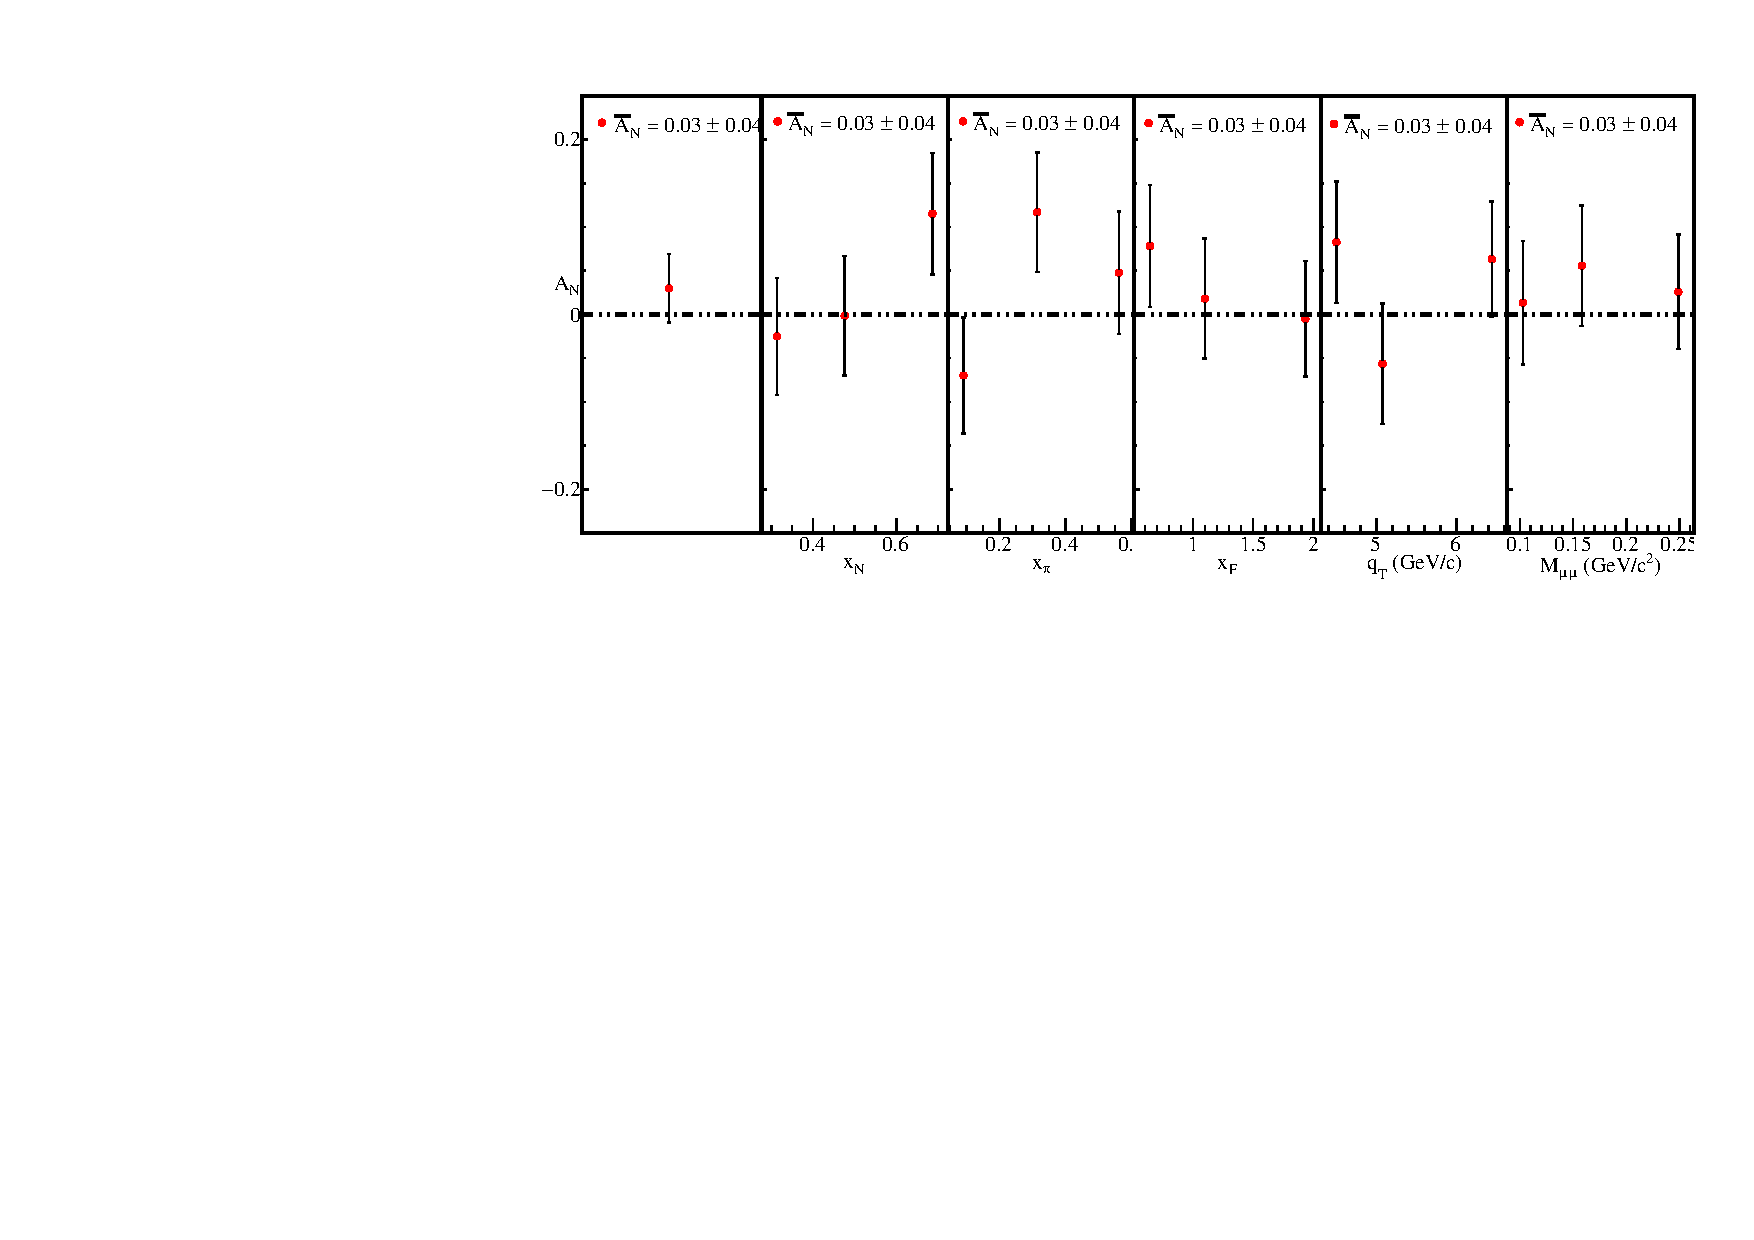
\includegraphics[width=\textwidth, trim=1.5cm 5cm 1.5cm 5cm,
      clip]{AN4TargGeom}
    %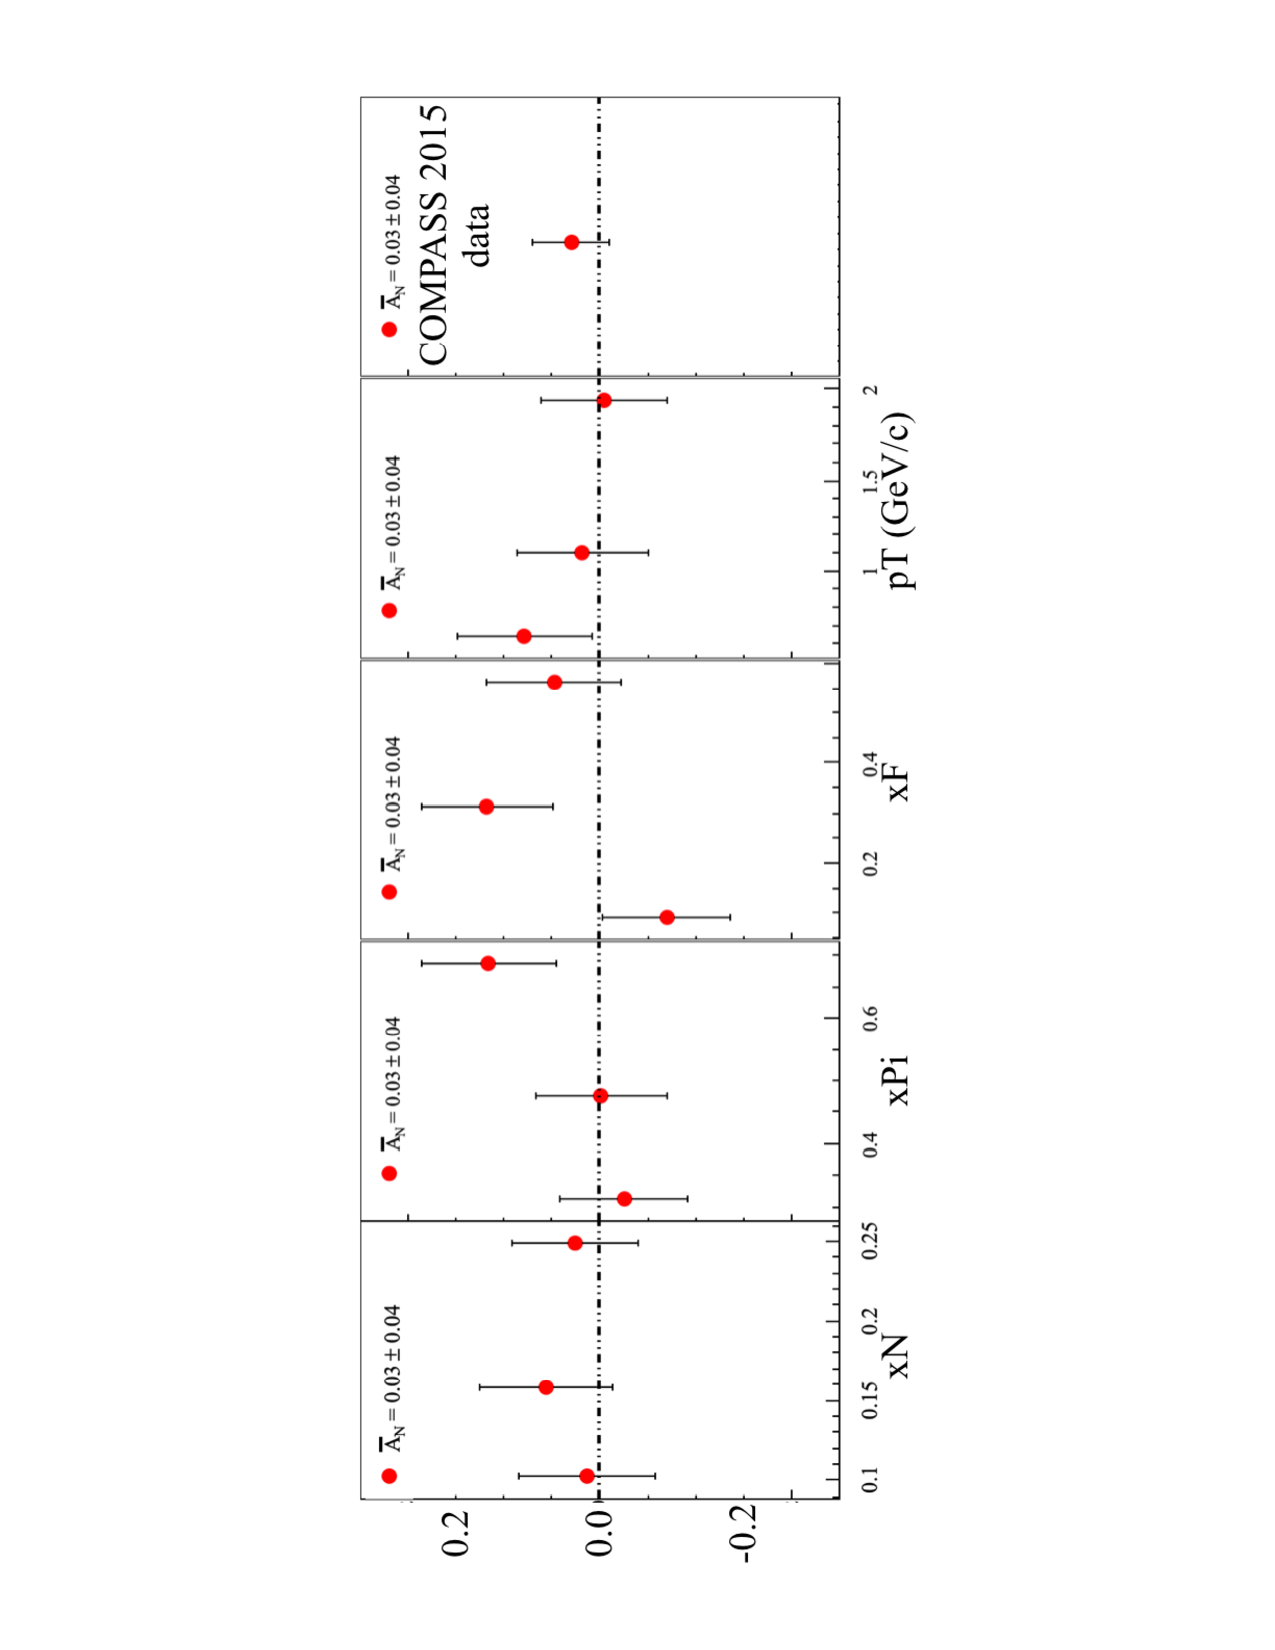
\includegraphics[width=0.9\textwidth]{ANgeom} %cleanup
    \caption{A$_N$ determined from the geometric mean method for each target}
    \label{fig::ANgeom}
  \end{center}
\end{figure}

\begin{figure}[h!t]
  \begin{center}
    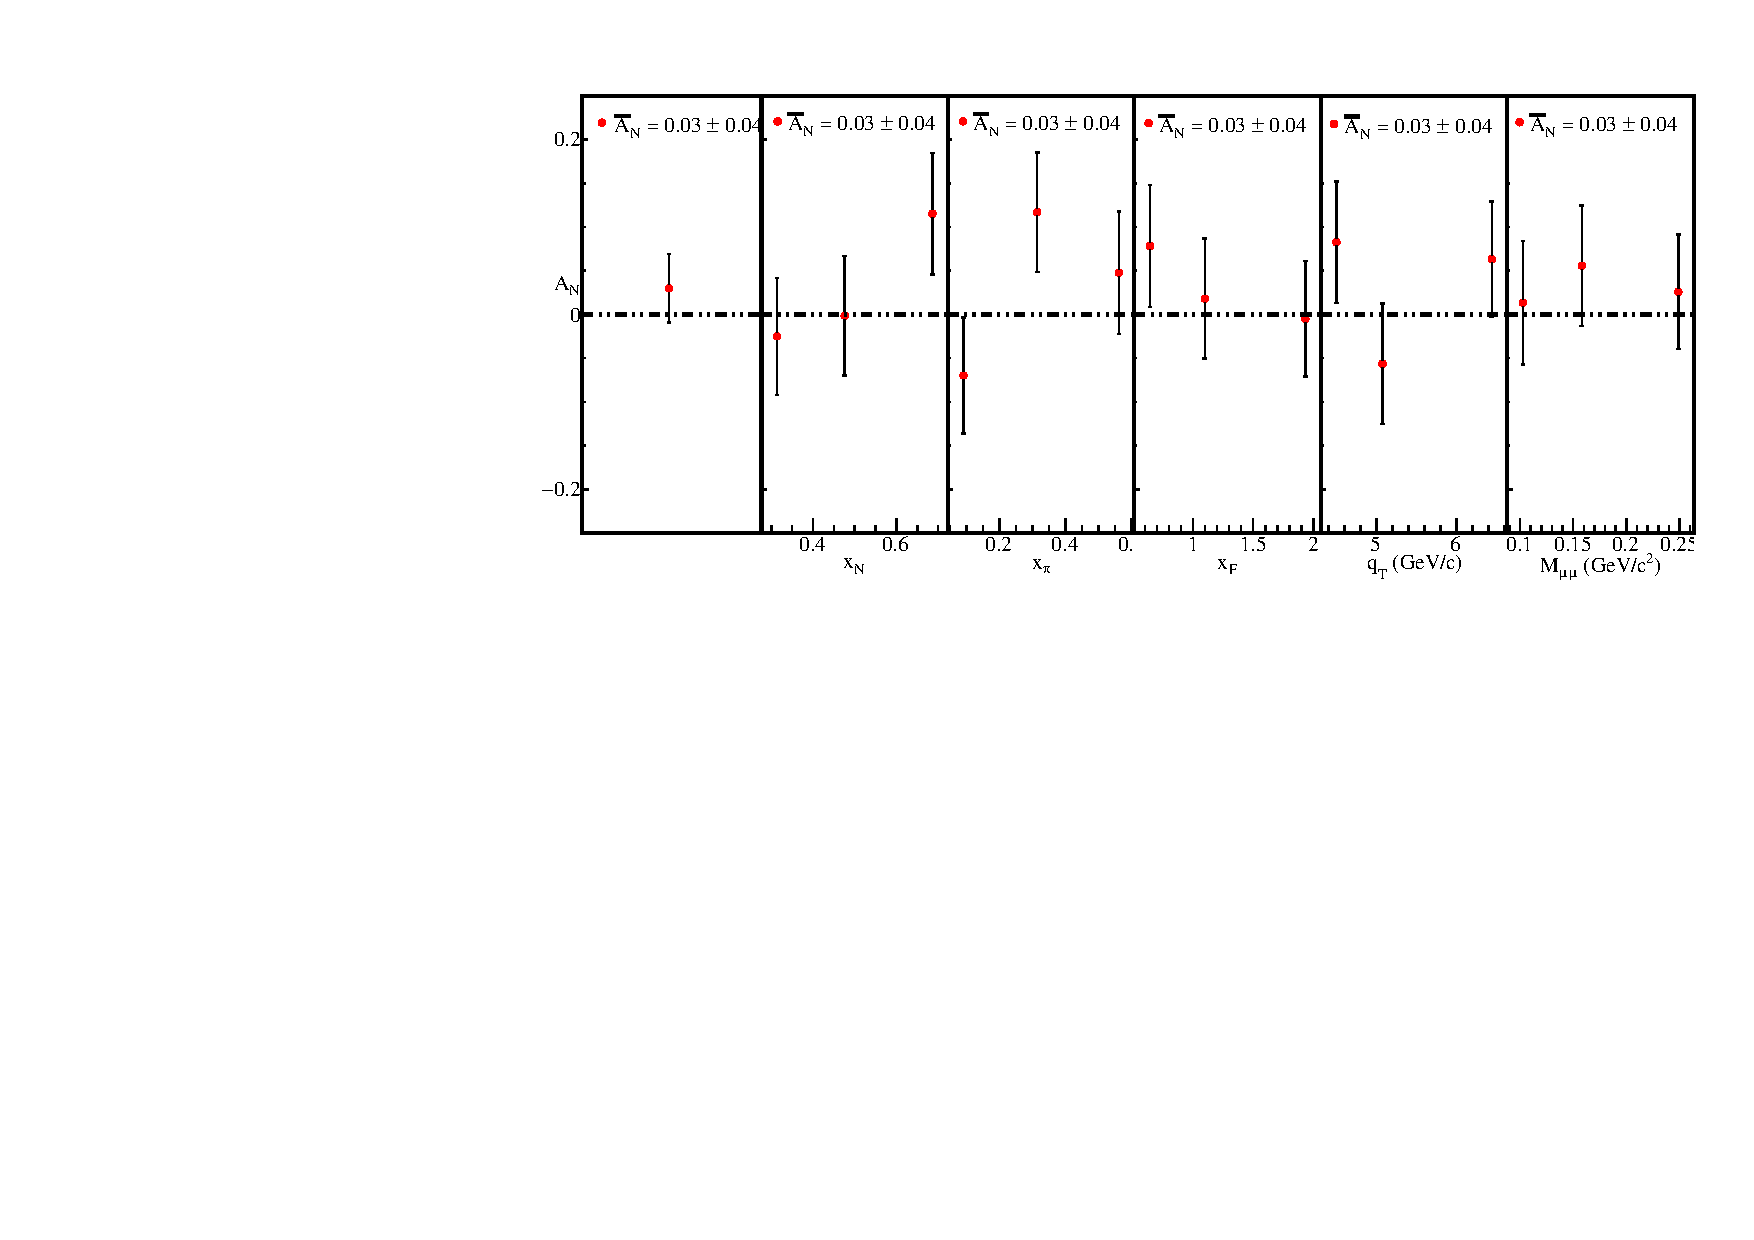
\includegraphics[width=\textwidth, trim=1.5cm 5cm 1.5cm 5cm,
      clip]{AN4TargGeom}
    \caption{A$_N$ determined by the geometric mean method using all targets
      simultaneously}
    \label{fig::AN4TargGeom}
  \end{center}
\end{figure}

\subsection{Comparison of results}


\section{Systematic Studies} \label{sec::systematics}
Several tests were performed to estimate the systematic uncertainty.  The final
systematic errors are determined by adding all non-zero systematic effects in
quadrature.  The impact from each source of systematic error is summarized in
Tab.~\ref{tab::sysError}.  List all test/systematic performed.....

\subsection{Period Compatibility}
The asymmetry calculated for each period in each kinematic bin is shown in
Fig.~\ref{allPhysBinned4Targ}.

\begin{figure}[h!t]
  \begin{center}
    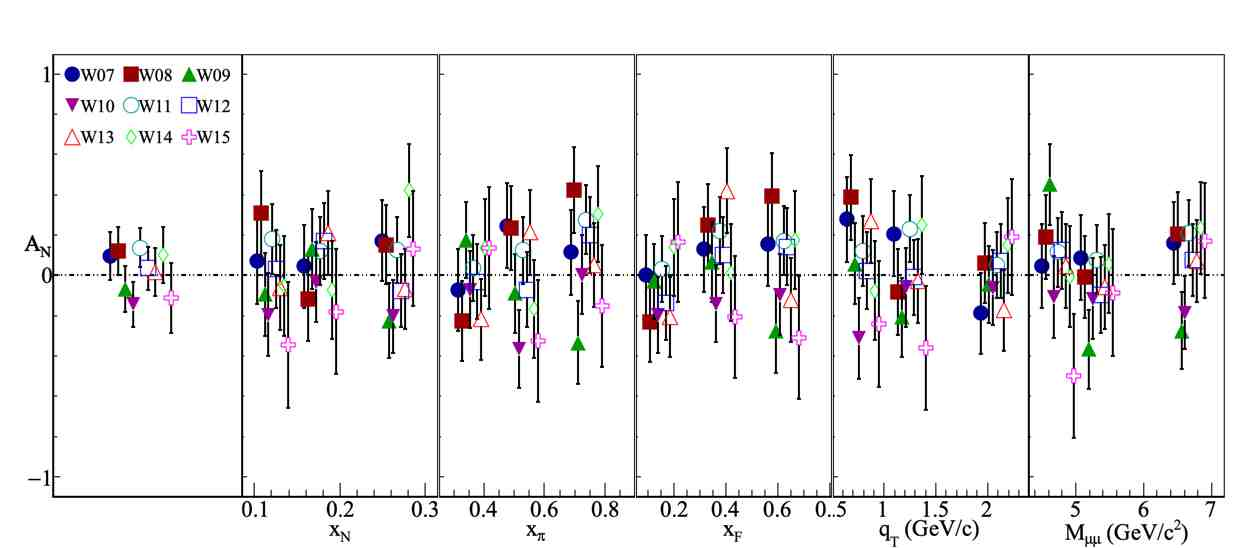
\includegraphics[width=\textwidth, trim=0cm 5cm 0cm 5cm,
      clip]{allPhysBinned4Targ}
    \caption{A$_N$ determined for each period}
    \label{fig::allPhysBinned4Targ}
  \end{center}
\end{figure}

\noindent
By eye the asymmetry fluctuations appear to be statistically compatible.  To
quantify the compatibility of the asymmetries between the periods, a pull
distribution is formed.  The pull value is defined as

\begin{equation}
  \label{eq::pull}
  \Delta\mathrm{A}_i =
  \frac{
    \mathrm{A}_i - \langle \mathrm{A} \rangle
  }{
    \sqrt{
      \sigma^2_{\mathrm{A}_i} - \sigma^2_{\langle \mathrm{A} \rangle}
    }
  },
\end{equation}

\noindent
and is determined for each period and kinematic bin.  There are therefore
3(number of bins)x5(number of kinematics)x9(number of periods) = 135 entries in
the pull distribution. This distribution is shown in Fig.~\ref{fig::pull4Targ}
along with a Gaussian fit.  If the asymmetries all come from the same parent
distribution then the pull distribution will be a Gaussian distribution with
zero mean and unit variance.  The discrepancy of the pull distribution from a
standard Gaussian distribution is used to determine systematic error as

\begin{equation}
  \frac{\sigma_{\mathrm{systematic}}}{\sigma_{\mathrm{statistical}}} =
  \sqrt{|\sigma^2_{\mathrm{pull}} - 1|} + \frac{\mu_{\mathrm{pull}}}{2}.
\end{equation}

\begin{figure}[h!t]
  \begin{center}
    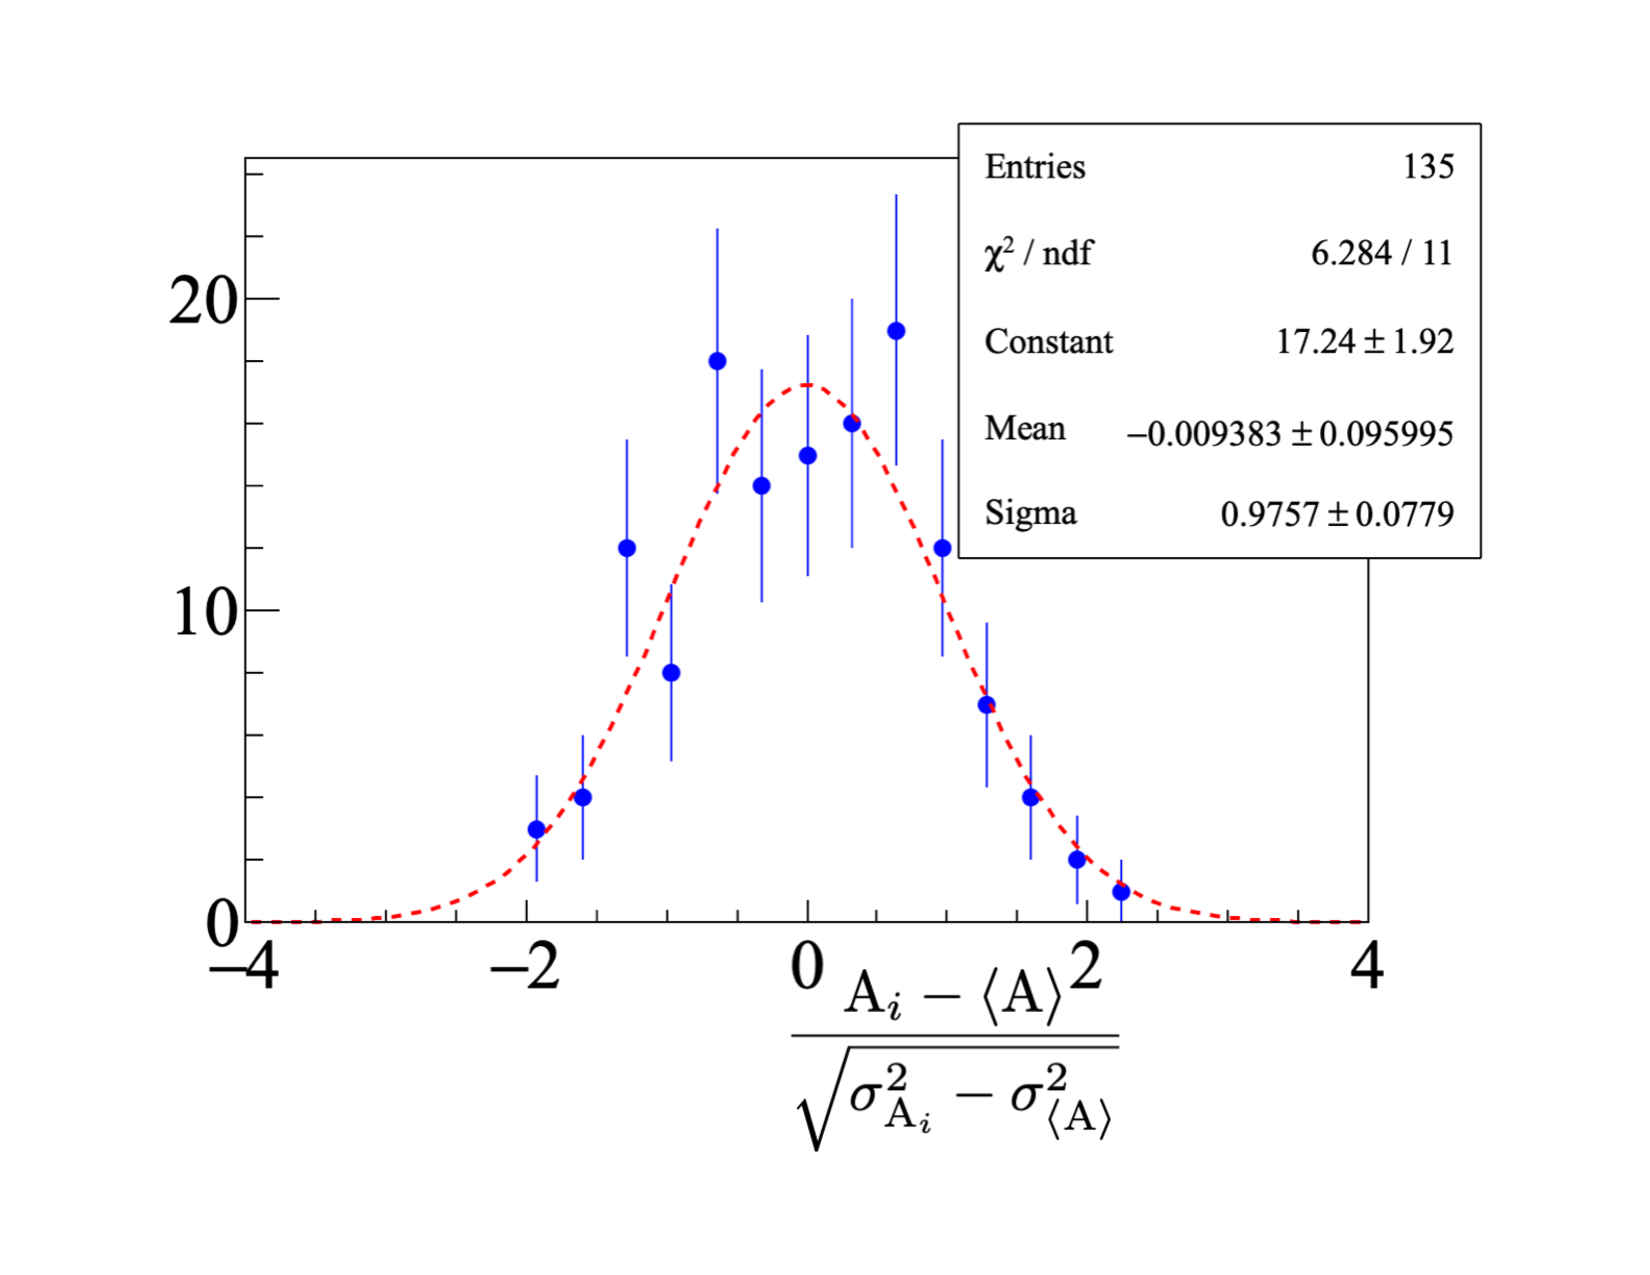
\includegraphics[width=0.8\textwidth, trim=0cm 0cm 0cm 2cm,clip]{pull4Targ}
    \caption{Pull distributions}
    \label{fig::pull4Targ}
  \end{center}
\end{figure}

\noindent
As the asymmetries in different kinematic bins are formed using the same data
set the asymmetries between kinematics are correlated.  For this reason an
uncorrelated pull distribution is form for each physics kinematic bin and also
compared with a standard Gaussian distribution.  These distributions are shown
in Fig.~\ref{fig::allPhysPulls4Targ} where there are now only 3(number of
bins)x9(number of periods) = 27 entries in each of the pull distributions.

\begin{figure}[h!t]
  \begin{center}
    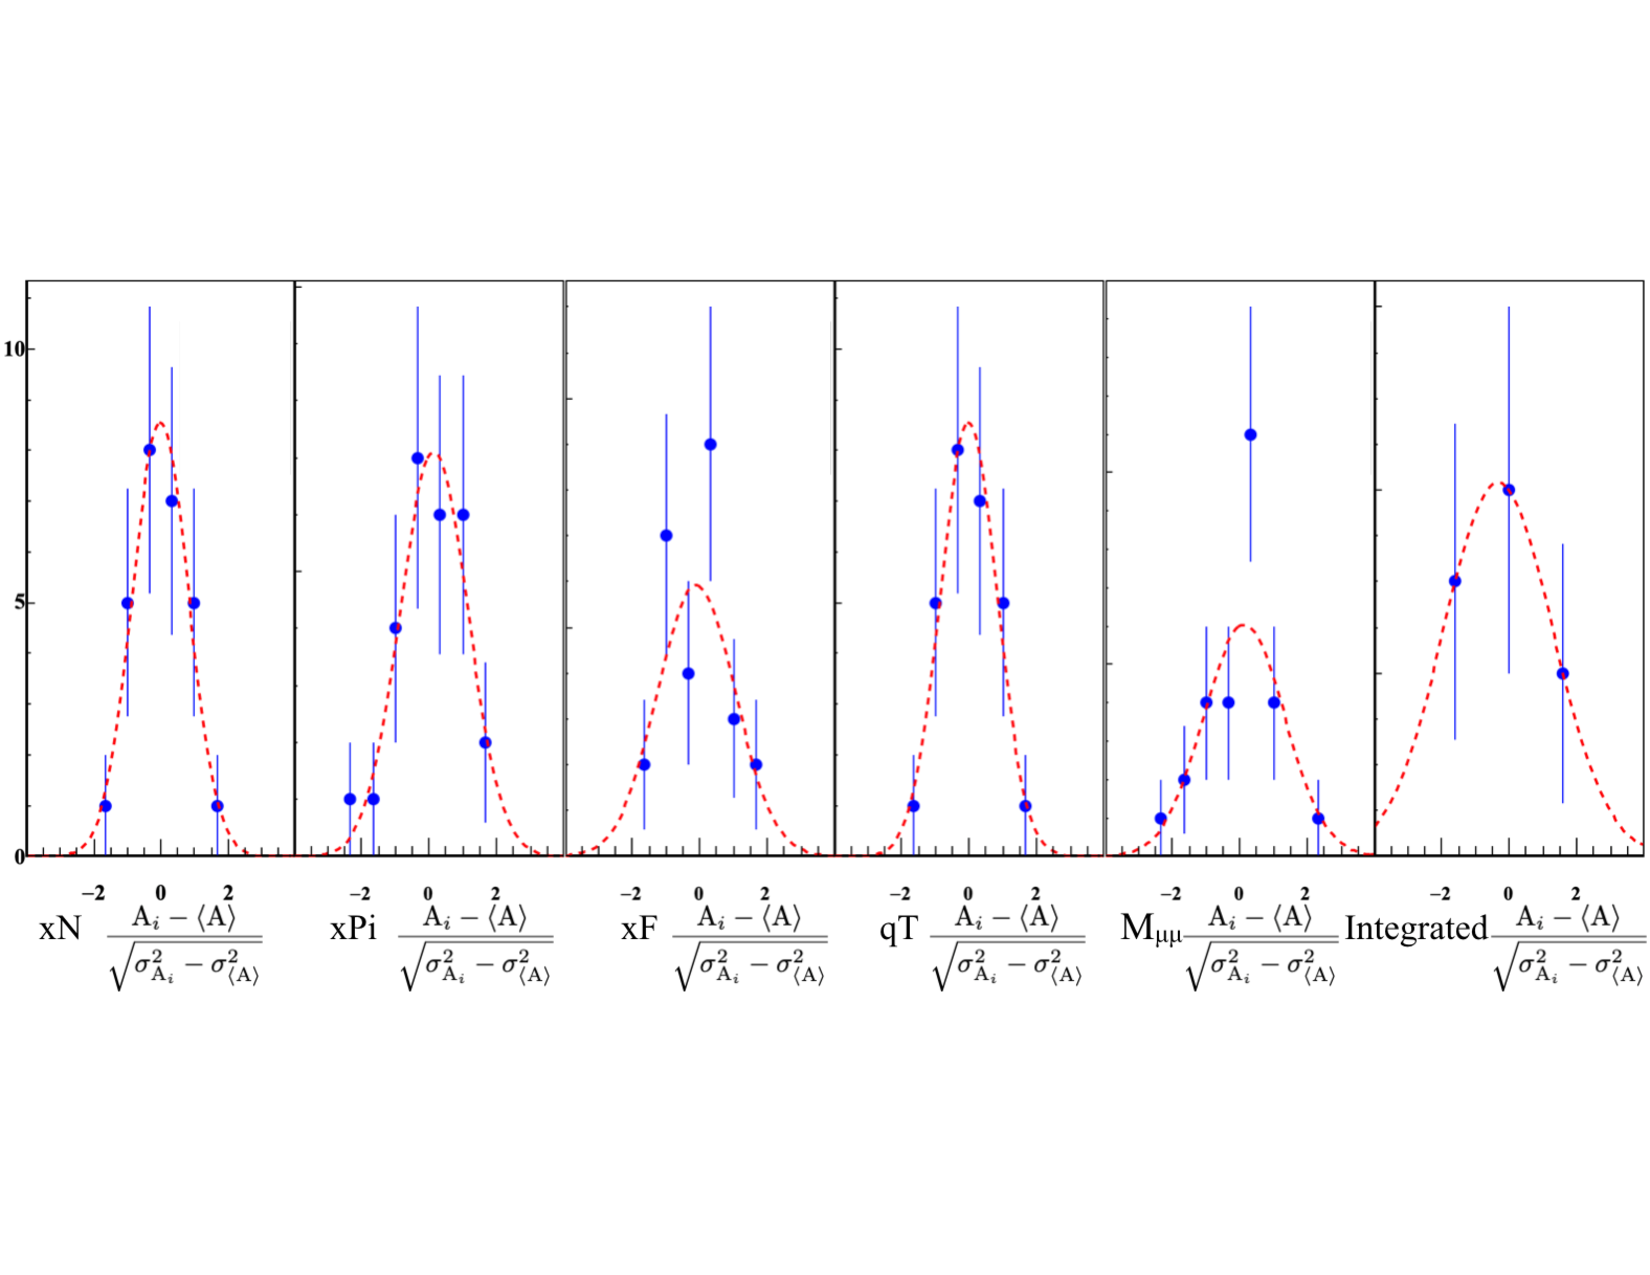
\includegraphics[width=\textwidth, trim=0cm 5cm 0cm 4cm,
      clip]{allPhysPulls4Targ}
    \caption{Pull distributions}
    \label{fig::allPhysPulls4Targ}
  \end{center}
\end{figure}

\noindent
The final systematic error from compatibility is...

\subsection{False Asymmetries}
\subsubsection{Acceptance From False Asymmetries}
As was pointed out in Sec.~\ref{sec::GeoMean} and
Sec.~\ref{sec::FourTargGeoMean}, the asymmetry measurement assumes the
acceptance does not change with time and therefore the acceptance ratios
Eq.~\ref{equ::accGeoMean} and Eq.~\ref{equ::acc4TargGeoMean} are unitary.  Any
deviation from unitary acceptance ratios is estimated with a false asymmetry and
the errors are included as systematic errors.  To determine if acceptance does
change with time, a false asymmetry is calculated where the only way the false
asymmetry could be non-zero is if acceptance changes with time.  This false
asymmetry for the four target geometric mean is

\begin{equation}
  \label{eqn::falseAcc}
  \begin{split}
    A_{\mathrm{N,False}} &= 
    \frac{1}{\mathrm{P}}
    \frac{
      \sqrt[4]{
        N_{\mathrm{up,Right}}^{\uparrow}N_{\mathrm{up, Left}}^{\downarrow}
        N_{\mathrm{down,Left}}^{\uparrow}N_{\mathrm{down, Right}}^{\downarrow}
      } -
      \sqrt[4]{
        N_{\mathrm{up,Left}}^{\uparrow}N_{\mathrm{up, Right}}^{\downarrow}
        N_{\mathrm{down,Right}}^{\uparrow}N_{\mathrm{down, Left}}^{\downarrow}
      }
    }{
      \sqrt[4]{
        N_{\mathrm{up,Right}}^{\uparrow}N_{\mathrm{up, Left}}^{\downarrow}
        N_{\mathrm{down,Left}}^{\uparrow}N_{\mathrm{down, Right}}^{\downarrow}
      } +
      \sqrt[4]{
        N_{\mathrm{up,Left}}^{\uparrow}N_{\mathrm{up, Right}}^{\downarrow}
        N_{\mathrm{down,Right}}^{\uparrow}N_{\mathrm{down, Left}}^{\downarrow}
      }
    }\\
    & =
    \frac{1}{\mathrm{P}}
    \frac{
      \alpha \sqrt[4]{\sigma_{Right}\sigma_{Left}\sigma_{Left}\sigma_{Right}} -
      \sqrt[4]{\sigma_{Left}\sigma_{Right}\sigma_{Right}\sigma_{Left}}
    }{
      \alpha \sqrt[4]{\sigma_{Right}\sigma_{Left}\sigma_{Left}\sigma_{Right}} +
      \sqrt[4]{\sigma_{Left}\sigma_{Right}\sigma_{Right}\sigma_{Left}}
    }\\
    & =
    \frac{1}{\mathrm{P}}
    \frac{
      \alpha - 1     
    }{
      \alpha + 1
    },
  \end{split}
\end{equation}

\noindent
where $\alpha$ is an acceptance ratio and is defined as

\begin{equation}
  \frac{
    \sqrt[4]{
      \mathrm{a}^{\uparrow}_{\mathrm{up,Saleve}}
      \mathrm{a}^{\downarrow}_{\mathrm{up,Saleve}}
      \mathrm{a}^{\uparrow}_{\mathrm{down,Jura}}
      \mathrm{a}^{\downarrow}_{\mathrm{down,Jura}}}
  }{
    \sqrt[4]{
      \mathrm{a}^{\uparrow}_{\mathrm{up,Jura}}
      \mathrm{a}^{\downarrow}_{\mathrm{up,Jura}}
      \mathrm{a}^{\uparrow}_{\mathrm{down,Saleve}}
      \mathrm{a}^{\downarrow}_{\mathrm{down,Saleve}}}
  }.
\end{equation}

\noindent
The kinematic dependencies of the false asymmetry are shown in
Fig.~\ref{fig::falseAacc} and the kinematic dependencies of the acceptance
ratio, $\alpha$, are shown in Fig.~\ref{fig::alpha}.

\begin{figure}[h!t]
  \begin{center}
    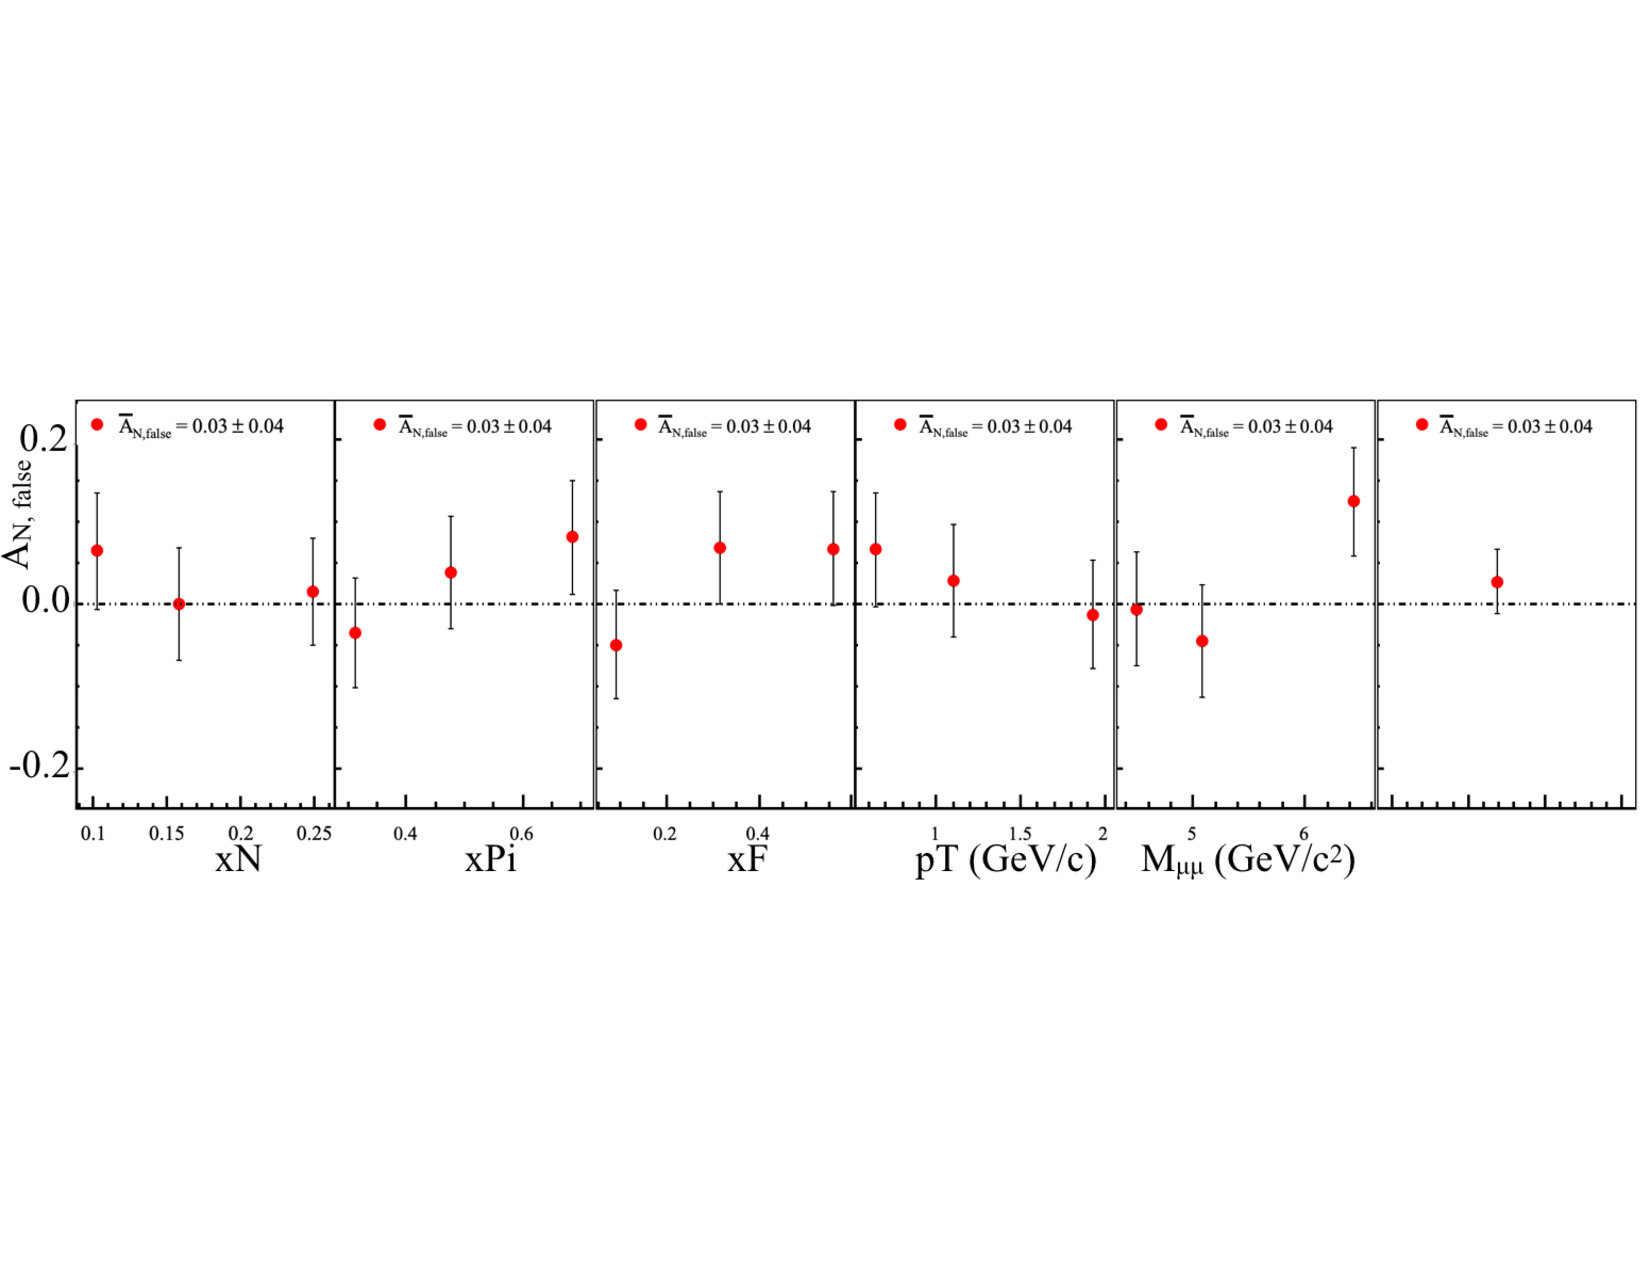
\includegraphics[width=\textwidth, trim=0cm 6.5cm 0cm 6.5cm,
      clip]{falseAacc}
    \caption{False asymmetry to estimate fluctuations in acceptance in time}
    \label{fig::falseAacc}
  \end{center}
\end{figure}

\begin{figure}[h!t]
  \begin{center}
    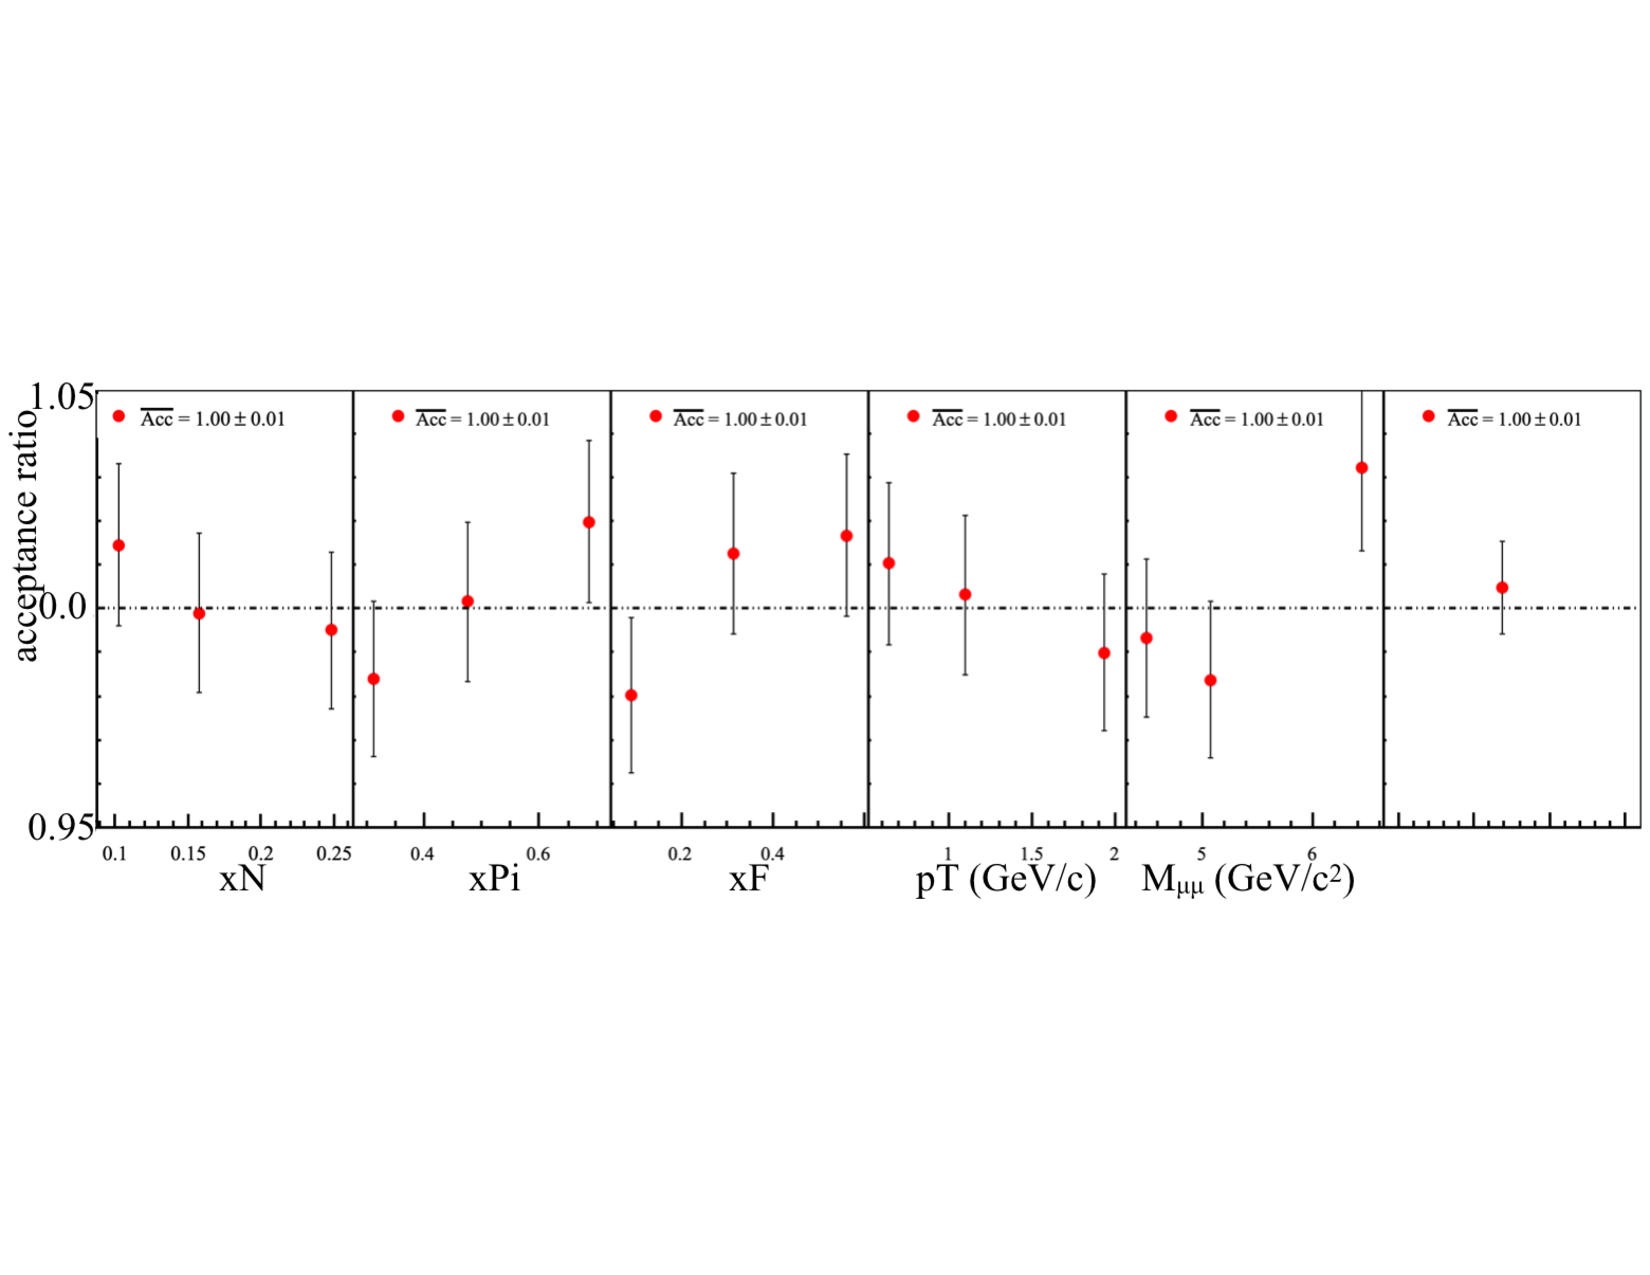
\includegraphics[width=\textwidth, trim=0cm 6cm 0cm 6cm,
      clip]{alpha4Targ}
    \caption{Acceptance ratio used to determine the systematic effects from
      acceptance changes in time}
    \label{fig::alpha}
  \end{center}
\end{figure}

\noindent
While $\alpha$ is an acceptance ratio it is not the same as the acceptance ratio
in the true asymmetry.  However $\alpha$ is similar to the true acceptance
ratio, $\kappa$, in that $\alpha$ will only be different from unity as a result
of time changes in the spectrometer.  Therefore it is assumed $\alpha$ can be
used as a good estimate of the true acceptance ratio.  The systematic error due
to acceptance fluctuations is determined as

\begin{equation}
  \delta\mathrm{A}_{\mathrm{N,systematic}} =
  \frac{1}{P} \Big(\frac{|\alpha-1|}{2} + \delta_{\frac{|\alpha-1|}{2}} \Big).
\end{equation}

\noindent
The kinematic dependence of the systematic error normalized to the statistical
error is show in Fig.~\ref{fig::accSysStat}.  The binned average systematic
error due to acceptance is 20\% of the statistical error.

\begin{figure}[h!t]
  \begin{center}
    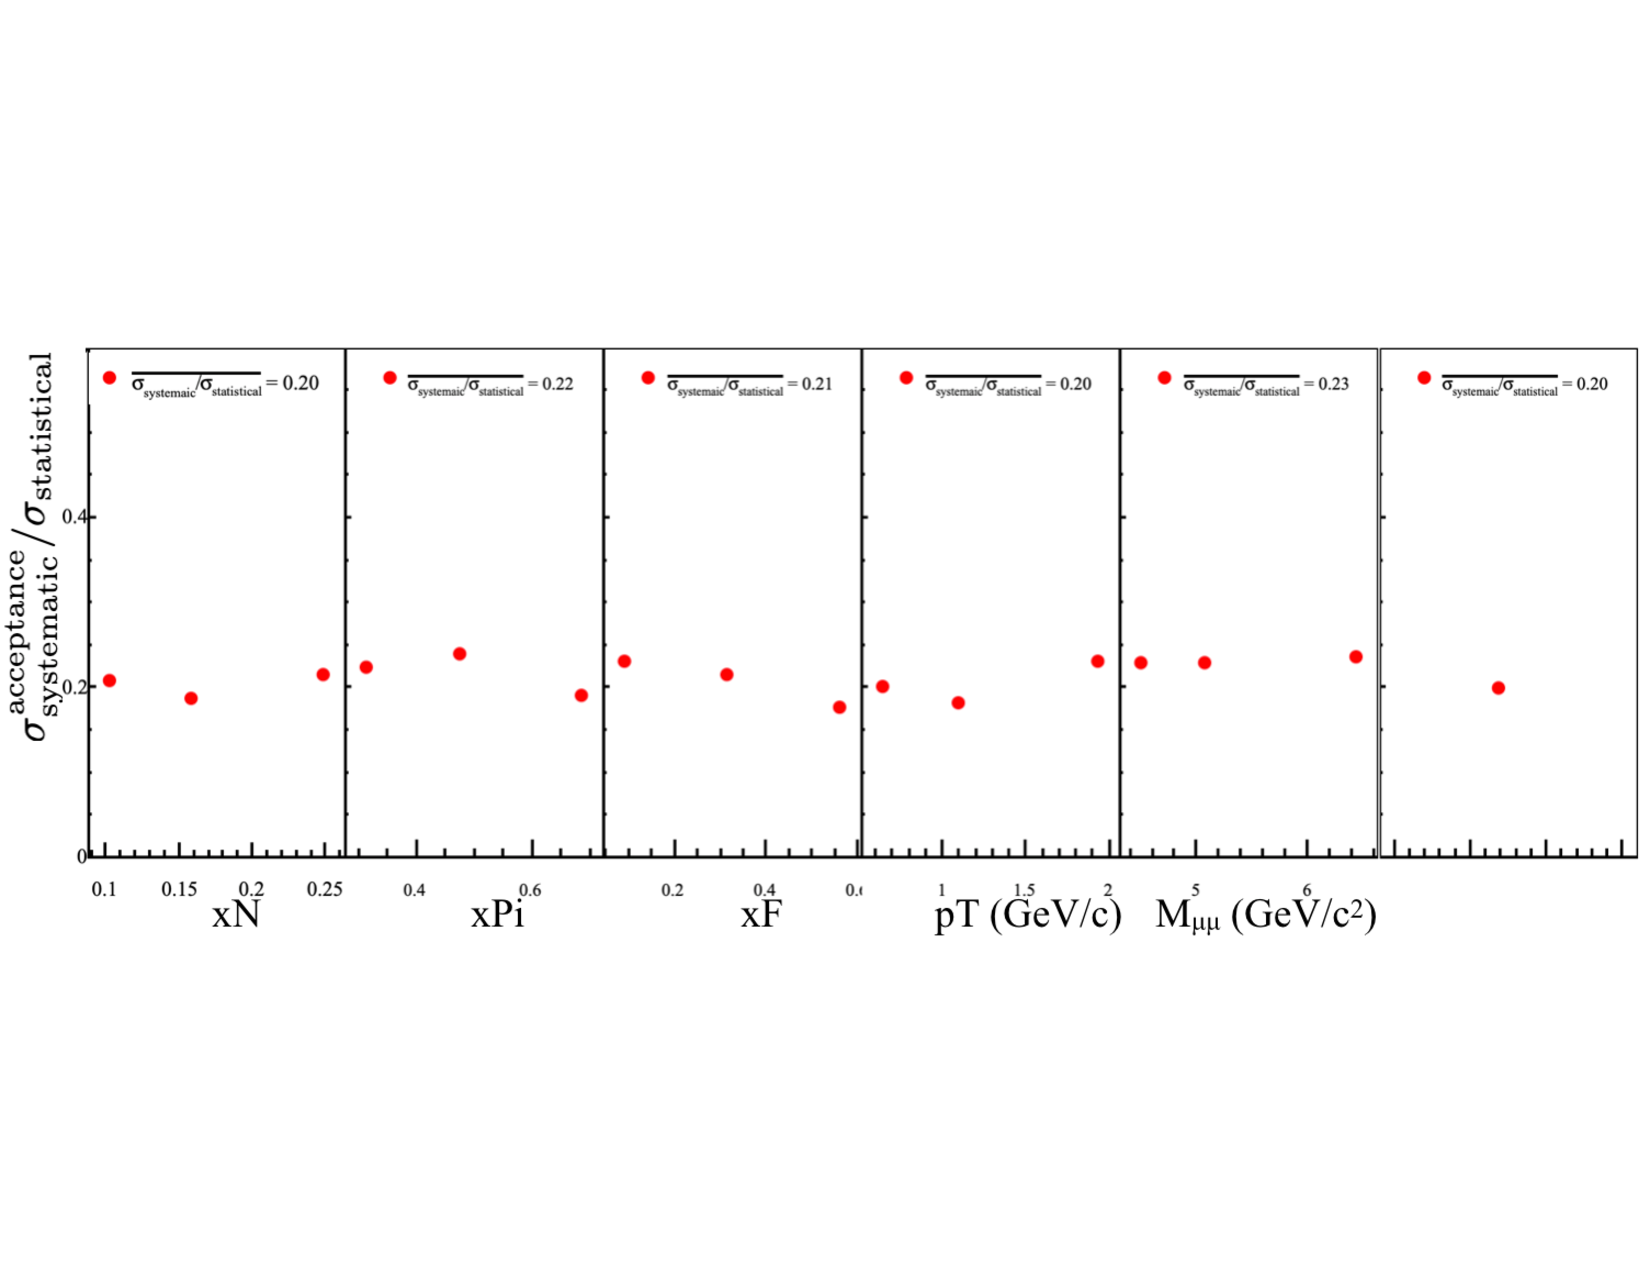
\includegraphics[width=\textwidth, trim=0cm 5cm 0cm 5cm,
      clip]{accSysStat}
    \caption{Systematic error due to acceptance effects}
    \label{fig::accSysStat}
  \end{center}
\end{figure}

\subsection{Further False Asymmetry Effects}
Although the list of systematic effects specifically studied is quite exhaustive
there is always the potential for other systematic effects not considered.
Studies of the changes in time from additional false asymmetries were performed
in an attempt to taken into all these other systematic effects.  All false
asymmetries considered must be constructed in such a way that the physical
process of interest cancels out.  A false asymmetry could therefore only be
non-zero from acceptance effects, luminosity or some other reason not
considered.  The additional false asymmetries constructed made in a way that
luminosity effects canceled out and acceptance effects were approximately
constant.  With these assumptions pull values from Eq.~\ref{eq::pull} should
from a standard Gaussian distribution.  Any deviation from a standard Gaussian
is conservatively taken as a systematic effect from some unknown cause.  The
additional studied false asymmetries are summarized in the following
~\ref{tab::additionalFA}.

\begin{enumerate}
  \label{tab::additionalFA}
\item A false asymmetry similar to Eq.~\ref{eqn::falseAcc} but with left and
  right counts shifted defined in Eq.~\ref{eqn::additionalfalseAsym}.
  
  \begin{equation}
    \label{eqn::additionalfalseAsym}
    \frac{1}{\mathrm{P}}
    \frac{
      \sqrt[4]{
        N_{\mathrm{up,Left}}^{\uparrow}N_{\mathrm{up,Right}}^{\downarrow}
        N_{\mathrm{down,Left}}^{\uparrow}N_{\mathrm{down,Right}}^{\downarrow}
      } -
      \sqrt[4]{
        N_{\mathrm{up,Right}}^{\uparrow}N_{\mathrm{up,Left}}^{\downarrow}
        N_{\mathrm{down,Right}}^{\uparrow}N_{\mathrm{down, Left}}^{\downarrow}
      }
    }{
      \sqrt[4]{
        N_{\mathrm{up,Left}}^{\uparrow}N_{\mathrm{up,Right}}^{\downarrow}
        N_{\mathrm{down,Left}}^{\uparrow}N_{\mathrm{down, Right}}^{\downarrow}
      } +
      \sqrt[4]{
        N_{\mathrm{up,Right}}^{\uparrow}N_{\mathrm{up,Left}}^{\downarrow}
        N_{\mathrm{down,Right}}^{\uparrow}N_{\mathrm{down, Left}}^{\downarrow}
      }
    }
  \end{equation}
\end{enumerate}

\subsection{Left/Right Event Migration}

\begin{table}[h!t]
  \centering
  \begin{tabular}{|c|c|}
    \hline Systematic error& \multirow{2}{9em}{$\langle
      \sigma_{\mathrm{systematic}}/\sigma_{\mathrm{statistical}}
      \rangle$}\\ & \\ \hline
    
    Period compatibility& 0.0\\ \hline

    Acceptance fluctuation& 0.2\\ \hline

    Total& 0.0\\\hline
    
  \end{tabular}
  \caption{Summary of systematic error impacts to the integrated asymmetry}
  \label{tab::sysError}
\end{table}
